\glsresetall

\section{Software Defined Networks}

\subsection{Evolution}

\subsubsection{RCP}
\subsubsection{4D}
\subsubsection{Ethane}
\subsubsection{OpenFlow}
\label{sec:related:openflow}
\subsubsection{Network Operating System}

%%%%%%%%%%%%%%%%%%%%%%%%%%%%%%%%%%%%%%%%%%%%%%%%%%
\glsresetall

\subsection{Fundamentals}
The \gls{sdn} architecture is not a standard. Rather it is an architectural approach to networking. It should be clear, by now, that SDN's are based on three essential design principles: decoupling of the control plane from the data plane; logically centralized network view;  versatile control of the data plane through an well established interface. 

So far \gls{sdn}  has not converged on well defined interfaces that we could use as reference to define its meta-architecture. 
However there are common elements throughout most of the existent \gls{sdn} literature. 
Consequently this section defines a common language  used throughout this document to refer to different SDN concepts. Following this,  we define the \gls{of} protocol details that will also be used throughout the document. This section can (and should) be used as reference throughout the text. 


\subsubsection{SDN Architecture}

\todo{cite rest}
\begin{figure}
  \centering
    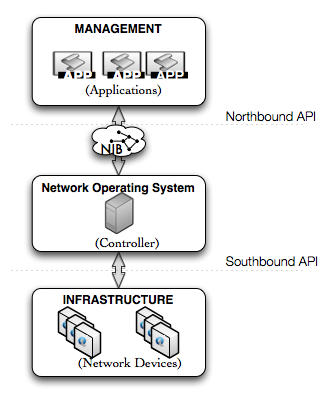
\includegraphics[width=\textwidth]{pic/related/sdn-stack}
  \caption{SDN Architecture}
  \label{fig:related:sdn-stack}
\end{figure}

The image is misleading in severals ways (for the sake of simplicity). First, the applications do not necessarily reside outside the control plane. They can be located in memory with the controller process whereby they cooperate to build the network state or configure the data plane devices. Second, the network state also does not necessarily reside outside the control plane in a data base. It could also be located in memory, or in extreme do not even exists (e.g., each application maintains its relevant state, state is acquired by consulting the data plane devices). 


The network logic operates in the \textbf{Management} plane. 
This plane defines the global network level objectives in the form of one or more (possibly) cooperative applications. 
Form a conceptual point of view  the applications interact with the controller through the north \gls{api}.  In practice this is not always true (explained further along the text). Usually a remote accessible api like an \gls{rest}\footnote{A web \gls{api} based on \gls{http} protocol.} over \gls{http} is used to this end. But other \glsplural{api} are just fine. In most control planes available applications can also subscribe to events in the controller through this \gls{api}. This is typically aplicable to in-memory applications but certainly does need to be the case. For this reason the image shows the north bound \gls{api} being used by the controller to  invoke operations in the applications. All the control planes referenced in this document allow this. In fact as we will see the event-oriented programming model is present throughout all the \gls{sdn} stack. The reason is simple, \gls{sdn} is event oriented from the get go, as network events are typically asynchronous in nature. 
 


In the \textbf{Control} plane resides the core logic that glues together all the \gls{sdn} architecture. This component is responsible for orchestrating the multiple applications available. Typically this implies two things: setting up the remote \textbf{North} \gls{api} (e.g., \gls{rest} web server) and also  maintaining in memory applications that cooperatively manage the network. Applications that build the most common network state are commonly provided by default in the controller, and usually operate in-memory. 
Regardless, the controller also maintains the shared state used (and modified by) applications. usmaintaing a platform where the in memory applications reside that cooperatively builds and maintain the \emph{Network State} with all the relevant information for the control platform in place (e.g., switch and link state,  topology, firewall rules, etc.,).  
This plane  is also in charge of the data plane communication, through South \gls{api}  that allows the data plane configuration (e.g., push/pull state from switches). Again, the South  \gls{api} can be event oriented whereby events are commonly topology information (i.e., link up, link down) and forwarding requests (e.g., flow tables misses in \gls{of}). 

Finally, the \textbf{Data} plane is where the network devices responsible for packet forwarding reside. Any device can be used (wireless access point, Ethernet Switch, router), as long as it implements the \emph{North} \gls{api}.\footnote{In practice a mixture of both \emph{North} bound enabled devices and normal devices is possible. Conceptually those networks are known as hybrid networks by the \gls{sdn} community.} We commonly refer to these elements as switches regardless  of they  functions perform in a standard mode (without the intervenction of a controller). 
Again, the \emph{South}  \gls{api}  operates in both directions. As such data plane elements can communicate with the controller. This allows them to perform forwarding requests on the controller or  update the controller view of the network (e.g., topology changes, INCLUDE MORE). 

The \textbf{West}/\textbf{East} \gls{api} are the same. They are applicable whenever  distributed control is employed (see Section~\ref{sec:related:distr-contr}). This \gls{api} is responsible for state distribution and controller to controller communication. It has two flows of communication for functions performed by the controller on another controller instance (e.g., push state, read state, install rules in another switch, etc.,) or in event oriented  implementations to receive events from other controllers (e.g., state has changed, new data plane event from a switch, MISSING ONE). 

There must be connectivity between the Control and the Data plane.
The connectivity may be  \textbf{in-bound} or \textbf{out-bound}. 
In the in-bound case the connectivity takes place over the
network used for data forwarding while in the out-bound case a
different and isolated network is used. Connectivity between these two layers require manual configuration of the Infrastructure components. 

\glsplural{sdn} can operate in two different models. In the  \textbf{Reactive} model a switch that does not known how to forward a packet can request the controller to ``takeover''. The controller can then take action (e.g., forward, drop, log)  and inform the switch. Typically (as shown in Fig.~\ref{fig:related:reactive}) the controller updates the switch with rules for both the packet and possibly packets that will follow it.  In constrast in a \textbf{Proactive} model the switch does not perform forwarding requests in the controller. Instead, the switch is configured according by the controller (according to the management networks objectives) and does not requests forwarding ``advice'' to the controller. We note however that the current \gls{sdn} technology is pliable enough to have both models. In fact one can choose between the two models for different types of traffic, or different periods of time in the same deployment. 

\subsubsection{OpenFlow}
Unfortunely, to make this document self contained we should clarify some technical aspects of the  \gls{of}  protocol. This section will briefly resume (and simplify) the most important characteristics of the protocol that should be used as reference for the remaining document. We note that the relevance of this protocol has already been covered in section~\ref{sec:related:openflow}.  


\gls{of} 
\begin{figure}
  \centering
  \includegraphics[width=\textwidth]{pic/related/openflow}
  \caption[Flow Request ]{Commonly, in an reactive model, the first packet of an flow for which there is no match is forwarded to the controller which evaluates it and decides the appropriate action. Normally it modifies the switch flow table such that the packets that follow do not have to go to the controller. }
  \label{fig:related:reactive}
\end{figure}

\begin{table}[ht]
  \centering
  \begin{tabular}[ht]{lll}
    Match Fields &  Instructions & Timeouts \\ \toprule 
    source MAC = 10:20:. \emph{AND}  protocol = ICMP  & port 2,3 & 5,10 ms \\ 
    source IP = 10.0.0.0/24  & port 1 &  0/0 \\
    source IP = 10.0.0.0/24 \emph{AND} protocol = TCP & controller & 0/0 \\ 
    any & controller & 0/0 \\ \bottomrule 
  \end{tabular}
  \caption[Openflow Flow Table]{Simplified representation of a flow table in OpenFlow switches.}
  \label{tab:related:openflow-flows}
\end{table}

Table~\ref{tab:related:openflow-flows} shows a simplified representation of an \gls{of} table present in the switch. 
The switch uses the match fields to find the intructions for any incoming packet. As oppossed to common devices which restrict tables to a small set of network packet headers (e.g., \gls{mac} for switches, \gls{ip} for routes) \gls{of} switches are able to match against 13 different headers (that can be combined with logical operators). Furthermore for some headers such as the \gls{ip} and \gls{mac} fields it can use bitmasks to match against a wide range of values. The table shows that the last two entries match against any host present in the $10.0.0.0/24$ network. Furthermore the switch can also match on the ports for each the packet arrives. Conflicting matches (i.e., a packet matches more than one entry in the table) are arbitrated by the priority associated with the rule (not show in the table). 

For each entry there is an associated instruction that the switch follows to forward the packet whenever it is able to find a match. Several instructions are available including: forward to port $x$, forward to controller, and drop the packet. As seen in the figure the instructions can be combined (the first entry forwards to two different ports). 

Each entry is removed from the table once one of the two private timeouts expire. There is an hard timeout which is never reset and an  idle timeout that is reset whenever an packet is matched against the entry. These timeouts are used by the controller to recycle and control the entries in the switch table. We note also that a value of 0  in the timeout means that it never expires. 

A \gls{of} switch table can be configured to forward non matching packets to the controller (as in our example in the last entry). Then, whenever an packet fails to match. 
%%%%%%%%%%%%%%%%%%%%%%%%%%%%%%%%%%%%%%%%%%%%%%%%%%
\glsresetall

\section{Physically Centralized Controllers}
\label{sec:related:phys-centr-contr}
Introduce default model. 

\subsection{Existent Work}
\subsubsection{NOX}
\subsubsection{Maestro}
\subsubsection{Beacon}

%%%%%%%%%%%%%%%%%%%%%%%%%%%%%%%%%%%%%%%%%%%%%%%%%%
\glsresetall
\subsection{Open Source Controllers}
\subsubsection{Existent Controllers}
\subsubsection{Controller Choice}

%%%%%%%%%%%%%%%%%%%%%%%%%%%%%%%%%%%%%%%%%%%%%%%%%%
\glsresetall
\section{Distributed Controllers}
\label{sec:related:distr-contr}
\subsection{Kandoo}
\label{sec:related:kandoo}
\subsection{HyperFlow}
\label{sec:related:hyperflow}
\subsection{Onix}
\label{sec:related:onix}

%%%%%%%%%%%%%%%%%%%%%%%%%%%%%%%%%%%%%%%%%%%%%%%%%%
\glsresetall
\section{Consistent Data Stores}


%%%%%%%%%%%%%%%%%%%%%%%%%%%%%%%%%%%%%%%%%%%%%%%%%%
\glsresetall
\section{Consistent Data Planes}


%%% Local Variables: 
%%% mode: latex
%%% TeX-master: "../PEI"
%%% End: 
